%% header.tex
%%
%% Copyright (C) 2016 - 2017  Dirk Eddelbuettel
%%
%% This file is part of samples-rmarkdown-metropolis repository.
%%
%% samples-rmarkdown-metropolis is free software: you can redistribute it
%% and/or modify it under the terms of the GNU General Public License as
%% published by the Free Software Foundation, either version 2 of the
%% License, or (at your option) any later version.
%%
%% samples-rmarkdown-metropolis is distributed in the hope that it will be
%% useful, but WITHOUT ANY WARRANTY; without even the implied warranty of
%% MERCHANTABILITY or FITNESS FOR A PARTICULAR PURPOSE.  See the GNU General
%% Public License for more details.
%%
%% You should have received a copy of the GNU General Public License along with
%% samples-rmarkdown-metropolis.  If not, see <http://www.gnu.org/licenses/>.

%% If you have the Fira font installed, to actually have it used it 
%% via rmarkdown you need to declare it here 
%\setsansfont[ItalicFont={Fira Sans Light Italic},BoldFont={Fira Sans},BoldItalicFont={Fira Sans Italic}]{Fira Sans Light}
%\setmonofont[BoldFont={Fira Mono Medium}]{Fira Mono}

%% You can set various Metropolis options via \metroset{} here
%\metroset{....}

%% You can redefine colours, mostly by borrowing from Beamer
\setbeamercolor{frametitle}{bg=gray}

%% You also use hyperref, and pick colors 
\hypersetup{colorlinks,citecolor=orange,filecolor=red,linkcolor=brown,urlcolor=blue}

%% when rendered with rmarkdown, somehow the unicode char for the dot
%% disappears so we redefine it here -- that is an older comments, seems font-specific
%\renewcommand{\textbullet}{$\cdot$}
%\renewcommand{\itemBullet}{▸}   % unicode U+25b8 'black right pointing small triangle'

%% The institute macro puts a small line for affiliation at the bottom
\institute{MSU Fisheries and Wildlife Graduate Symposium} 

%% We can also place a logo
\titlegraphic{\hfill
\includegraphics[height=2cm]{images/contlimno.png}}

%%% Local Variables:
%%% mode: latex
%%% TeX-master: t
%%% End:

\def\begincols{\begin{columns}}
\def\endcols{\end{columns}}
\def\begincol{\begin{column}}
\def\endcol{\end{column}}

\usetikzlibrary{decorations.pathmorphing,calc}
\def\lakediagramgreen{
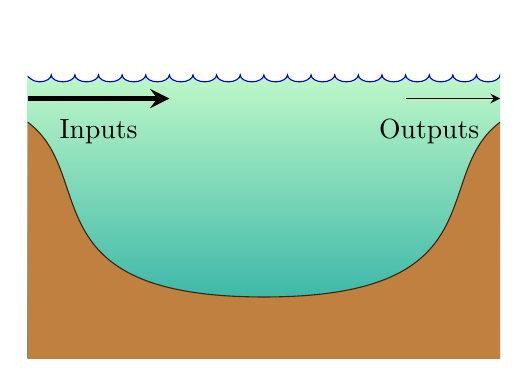
\begin{tikzpicture}[scale = 0.6]
% https://tex.stackexchange.com/questions/95044/create-diagrams-in-latex-with-tikz

% Define some reference points 
% The figure is drawn a bit bigger, and then clipped to the following dimensions:
\coordinate (clipping area) at (10, 7);
\clip (0,0) rectangle (clipping area);

% Next reference points are relative to the lower left corner of the clipping area
\coordinate (water level) at (0, 6);
\coordinate (bottom)      at (5, 1.3);     % (bottom of the pit)
\coordinate (ground1)     at (0, 5);       % (left shore)
\coordinate (ground2)     at (10, 5);      % (right shore)

% Coordinates of the bigger area really drawn
\coordinate (lower left)  at ([xshift=-5mm, yshift=-5mm] 0,0);
\coordinate (upper right) at ([xshift=5mm,  yshift=5mm] clipping area);

% Draw the water and ripples
\draw [draw=blue!80!black, decoration={bumps, mirror, segment length=6mm}, decorate,
     bottom color=cyan!60!black, top color=green!20!white] 
  (lower left) rectangle (water level-|upper right);

% Draw the ground
\draw [draw=brown!30!black, fill=brown] 
  (lower left) -- (lower left|-ground1)  --
  (ground1) .. controls ($(ground1)!.3!(bottom)$) and (bottom-|ground1) ..
  (bottom) .. controls (bottom-|ground2) and ($(ground2)!.3!(bottom)$) .. 
  (ground2) -- (ground2-|upper right) -- (lower left-|upper right) -- cycle;

% \draw[dotted](0,0) rectangle (clipping area);

% labels
\draw[>=stealth, ->, line width = 0.7mm] (0, 5.5) -- (3, 5.5) node at (1.5, 4.8) {Inputs};
\draw[>=stealth, ->, line width = 0.2mm] (8, 5.5) -- (10, 5.5) node at (8.5, 4.8) {Outputs};

\end{tikzpicture}
}

\def\lakediagramblue{
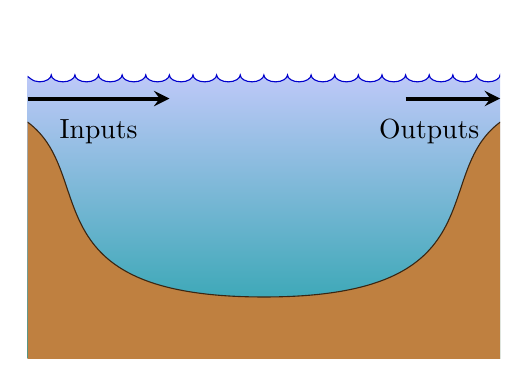
\begin{tikzpicture}[scale = 0.6]
% https://tex.stackexchange.com/questions/95044/create-diagrams-in-latex-with-tikz

% Define some reference points 
% The figure is drawn a bit bigger, and then clipped to the following dimensions:
\coordinate (clipping area) at (10, 7);
\clip (0,0) rectangle (clipping area);

% Next reference points are relative to the lower left corner of the clipping area
\coordinate (water level) at (0, 6);
\coordinate (bottom)      at (5, 1.3);     % (bottom of the pit)
\coordinate (ground1)     at (0, 5);       % (left shore)
\coordinate (ground2)     at (10, 5);      % (right shore)

% Coordinates of the bigger area really drawn
\coordinate (lower left)  at ([xshift=-5mm, yshift=-5mm] 0,0);
\coordinate (upper right) at ([xshift=5mm,  yshift=5mm] clipping area);

% Draw the water and ripples
\draw [draw=blue!80!black, decoration={bumps, mirror, segment length=6mm}, decorate,
     bottom color=cyan!60!black, top color=blue!20!white] 
  (lower left) rectangle (water level-|upper right);

% Draw the ground
\draw [draw=brown!30!black, fill=brown] 
  (lower left) -- (lower left|-ground1)  --
  (ground1) .. controls ($(ground1)!.3!(bottom)$) and (bottom-|ground1) ..
  (bottom) .. controls (bottom-|ground2) and ($(ground2)!.3!(bottom)$) .. 
  (ground2) -- (ground2-|upper right) -- (lower left-|upper right) -- cycle;

% \draw[dotted](0,0) rectangle (clipping area);

% labels
\draw[>=stealth, ->, line width = 0.5mm] (0, 5.5) -- (3, 5.5) node at (1.5, 4.8) {Inputs};
\draw[>=stealth, ->, line width = 0.5mm] (8, 5.5) -- (10, 5.5) node at (8.5, 4.8) {Outputs};

\end{tikzpicture}
}

\def\connectivitydiagram{
\begin{columns}

\begin{column}{0.25\textwidth}
    
\begin{tikzpicture}
      \draw [-,ultra thick, cyan] (-1,3) to [out=270,in=180] (0.2,2) to [out=0,in=90] (0,0.3) to [out=90,in=0] (0,-1) to [out=90,in=0] (0.2,-2) to [out=180,in=90] (-1,-3);
      \draw[cyan, ultra thick, domain=0:350, smooth cycle, fill=cyan,yshift=20] plot (\x:0.5+rnd*0.25);
      \draw[cyan, ultra thick, domain=0:350, smooth cycle, fill=cyan,yshift=-50] plot (\x:0.8+rnd*0.5);
      \node at (0,-1.7) {Secondary};
    \end{tikzpicture}
  \end{column}
  
  \begin{column}{0.25\textwidth}
    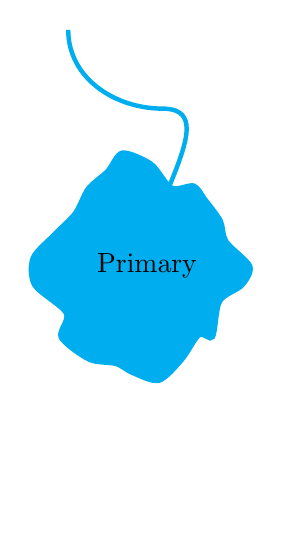
\begin{tikzpicture}
      \draw [-,ultra thick, cyan] (-1,3) to [out=270,in=180] (0.2,2) to [out=0,in=90] (0,0);
      \draw[cyan, ultra thick, domain=0:350, smooth cycle, fill=cyan] (0,-3) plot (\x:1+rnd*0.5);
      \node at (0, 0) {Primary};
    \end{tikzpicture}
  \end{column}
  
  \begin{column}{0.25\textwidth}
  
\begin{tikzpicture}
      \draw [-,ultra thick, cyan] (0,0) to [out=90,in=0] (0.2,-2) to [out=180,in=90] (-1,-3);
      \draw[cyan, ultra thick, domain=0:350, smooth cycle, fill=cyan] (0,3) plot (\x:1+rnd*0.5);
      \node at (0, 0) {Headwater};
    \end{tikzpicture}
  \end{column}
  
  \begin{column}{0.25\textwidth}
    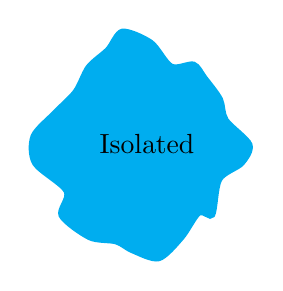
\begin{tikzpicture}
      \draw[cyan, ultra thick, domain=0:350, smooth cycle, fill=cyan] plot (\x:1+rnd*0.5);
      \node at (0, 0) {Isolated};
    \end{tikzpicture}
  \end{column}
  
\end{columns}

}

\usepackage{subfiles}
\usepackage{pbox}
\usepackage{multirow}
\usepackage{tabularx}
\usepackage{xcolor,colortbl}

\usepackage{array}
\newcolumntype{L}[1]{>{\raggedright\let\newline\\\arraybackslash\hspace{0pt}}m{#1}}
\newcolumntype{C}[1]{>{\centering\let\newline\\\arraybackslash\hspace{0pt}}m{#1}}
\newcolumntype{R}[1]{>{\raggedleft\let\newline\\\arraybackslash\hspace{0pt}}m{#1}}

\newcolumntype{K}[1]{%
 >{\vbox to 5ex\bgroup\vfill\centering}%
 p{#1}%
 <{\egroup}} 